%-------------------------
% Resume in Latex
% Author : Sourabh Bajaj
% Website: https://github.com/sb2nov/resume
% License : MIT
%------------------------

\documentclass[11pt]{article}
% \usepackage[a4paper, margin=3in]{geometry}
% \usepackage{geometry}

\usepackage{latexsym}
\usepackage[empty]{fullpage}
\usepackage{titlesec}
\usepackage{marvosym}
\usepackage[usenames,dvipsnames]{color}
\usepackage{verbatim}
\usepackage{enumitem}
\usepackage{lipsum}
%\usepackage[pdftex]{hyperref}
\usepackage{fancyhdr}
\usepackage{wrapfig}
\usepackage{graphicx, tikz, geometry}
\usepackage{float}

\usepackage[pdftex, colorlinks=true, linkcolor=blue, urlcolor=blue, citecolor=blue]{hyperref}

\newcommand{\twocol}[2]{%
  \noindent
  \begin{minipage}[t]{0.655\linewidth}\raggedright #1\end{minipage}\hfill
  \begin{minipage}[t]{0.330\linewidth}\raggedright #2\end{minipage}%
}

\newcount\myloopcounter

\newcommand{\repeatit}[2][10]{%
  \myloopcounter0% initialize the loop counter
  \loop\ifnum\myloopcounter < #1 % Test if the loop counter is < #1
  #2%
  \advance\myloopcounter by 1 % 
  \repeat % start again
}

\pagestyle{fancy}
\fancyhf{} % clear all header and footer fields
\fancyfoot{}
\renewcommand{\headrulewidth}{0pt}
\renewcommand{\footrulewidth}{0pt}

% Adjust margins
\addtolength{\oddsidemargin}{-1.150in}
\addtolength{\evensidemargin}{-1.150in}
\addtolength{\textwidth}{2.275in}
\addtolength{\topmargin}{-1.13in}
\addtolength{\textheight}{2.8in}

\urlstyle{same}

\raggedbottom
\raggedright
\setlength{\tabcolsep}{0in}

% Sections formatting
\titleformat{\section}{
  \vspace{-4pt}\scshape\raggedright\large
}{}{0em}{}[\color{black}\titlerule \vspace{-5pt}]

%-------------------------
% Custom commands
\newcommand{\resumeItem}[2]{
  \item\small{
    \textbf{#1}{: #2 \vspace{-2pt}}
  }
}

\newcommand{\resumeSubheading}[4]{
  \vspace{-1pt}\item
    \begin{tabular*}{0.97\textwidth}{l@{\extracolsep{\fill}}r}
      \textbf{#1} & #2 \\
      \textit{} & \textit{\small #4} \\
    \end{tabular*}\vspace{-12pt}
    \textit{\small\begin{minipage}{0.73\textwidth}#3\end{minipage}}
    \vspace{-5pt}
}

\newcommand{\resumeSubItem}[2]{\resumeItem{#1}{#2}\vspace{-4pt}}

\renewcommand{\labelitemii}{$\circ$}

\newcommand{\resumeSubHeadingListStart}{\begin{itemize}[leftmargin=*]}
\newcommand{\resumeSubHeadingListEnd}{\end{itemize}}
\newcommand{\resumeItemListStart}{\begin{itemize}}
\newcommand{\resumeItemListEnd}{\end{itemize}\vspace{-5pt}}

%-------------------------------------------
%%%%%%  CV STARTS HERE  %%%%%%%%%%%%%%%%%%%%%%%%%%%%


\begin{document}

%----------HEADING-----------------
\begin{tabular*}{\textwidth}{l@{\extracolsep{\fill}}r}
  \textbf{{\Large William Bille Meyling}}\\ \textbf{E-mail}: \href{mailto:williambillemeyling@gmail.com}{williambillemeyling@gmail.com} \textbf{Mobile}: +45 24445317\\
  \textbf{Github}: \href{https://github.com/willthbill}{https://github.com/willthbill} \textbf{LinkedIn}: \href{https://www.linkedin.com/in/williambillemeyling}{https://bit.ly/linkedin-wbm} \\
  \textbf{Personal website}: \href{https://willthbill.dev}{https://willthbill.dev}\\
\end{tabular*}

%-----------BIO-----------------
\begin{tikzpicture}[overlay,remember picture]
 \node[anchor=north west,inner sep=0pt]at ([xshift=17.0cm,yshift=-0.4cm]current page.north west) {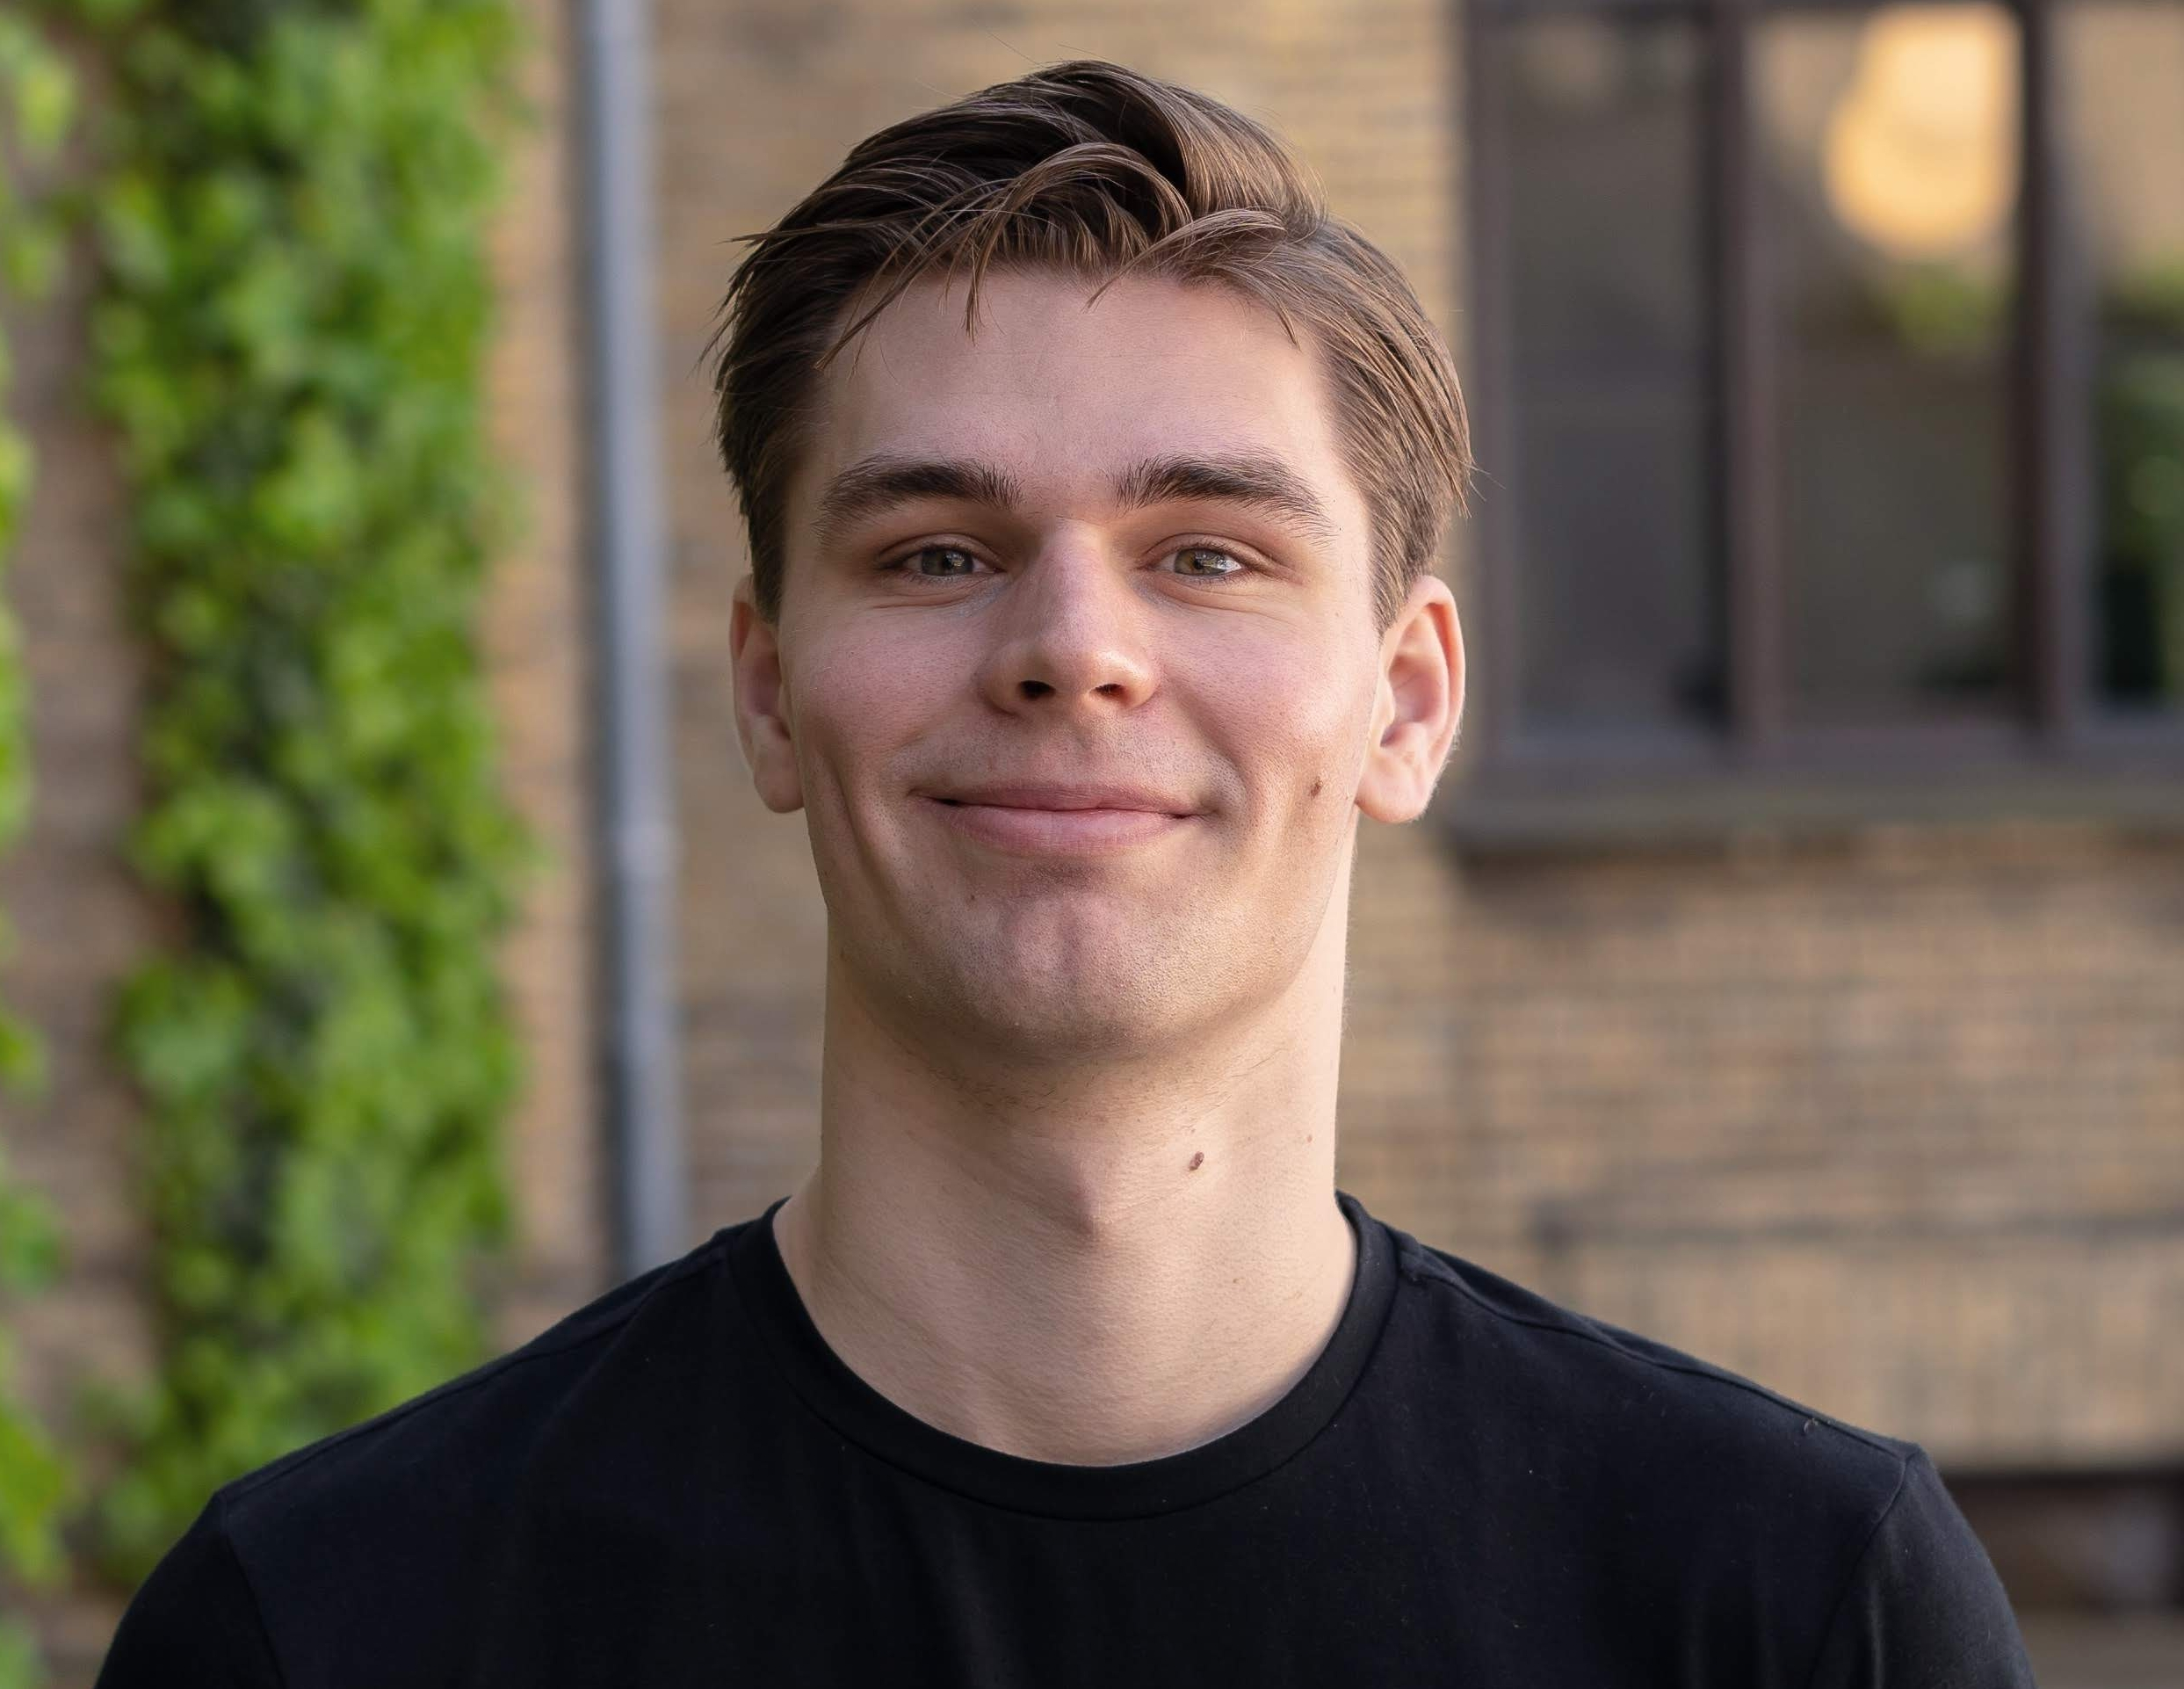
\includegraphics[width=4cm]{me_cropped.jpg}};
\end{tikzpicture}

\begin{minipage}{15.8cm}
Software engineer and ex-founder with a strong background in algorithms and high-performance systems, skilled at writing clean, correct, efficient code quickly. Fluent in English and Danish.
\end{minipage}
\vspace{-6pt}

\section{Skills}
\resumeSubHeadingListStart

  \resumeSubItem{Algorithms and optimization}
    {\footnotesize{IOI, ICPC EUC, national champion. Skilled at writing correct, efficient code quickly.}}

  \resumeSubItem{Software design}
    {\footnotesize{Designing modular, maintainable systems. Experience with projects in the 10k–200k LOC range.}}

  \resumeSubItem{High-performance systems}
    {\footnotesize{Rust and Python. Built ultra-fast real-time data pipelines and ML inference in production.}}

  \resumeSubItem{Data engineering}
    {\footnotesize{Hands-on with Rust, Python, Polars, S3, Postgres, Prefect, and servers. Built and maintained datasets, performed feature engineering, and created dashboards for trading signal analysis.}}

  \resumeSubItem{Bash, Linux \& DevOps}
    {\footnotesize{Comfortable running servers, writing automation scripts, using Docker, and handling basic security tasks.}}

\resumeSubHeadingListEnd

%\vspace{2mm}
%\noindent\textbf{Additional experience (not core expertise):}
%\vspace{-4pt}
\resumeSubHeadingListStart

  \resumeSubItem{Machine learning}
    {\footnotesize{Used PyTorch for small neural nets, LGBM, and Hugging Face models; integrated models into pipelines.}}

  \resumeSubItem{AI agents}
    {\footnotesize{Built full-stack AI agent apps using Lovable and LangGraph; experience interacting with LLMs via APIs.}}

  \resumeSubItem{Full-stack development}
    {\footnotesize{Capable of building complete applications (frontend + backend + DB).}}

  \resumeSubItem{Currently learning}
    {\footnotesize{CUDA, Infrastructure-as-Code, observability platforms (e.g., Datadog).}}

\resumeSubHeadingListEnd


%-----------EDUCATION-----------------
\section{Education}
  \resumeSubHeadingListStart
    \resumeSubheading
      {University of Copenhagen}{Sep. 2020 - Aug. 2023}
      {Bachelor of Science (BSc) in Computer Science. Grade: 12 (equivalent to A+)}{}
  \resumeSubHeadingListEnd
  
%-----------EXPERIENCE-----------------
\section{Experience}
  \resumeSubHeadingListStart
    \resumeSubheading
      {Co-founder of Dafnis ApS}{Aug. 2023 - Jun. 2025}
      {\footnotesize{A fully automated power trading firm using machine learning and algorithms to trade power across Europe. Utilizing a modern, high-performance tech stack, written in Rust. Responsible for fast data pipelines and backtesting systems.}}{}
    \resumeSubheading
      {Researcher at University of Copenhagen}{Sep. 2023 - Feb. 2024}
      {\footnotesize{Using MILP in Computational Geometry. C++.}}{}
    \resumeSubheading
    {Full-stack Student developer at Jobindex}{Feb. 2021 - Jan. 2022}
      {\footnotesize{Tools: MySQL, Perl, Vue.js}}{}
    \resumeSubheading
      {Trainer at Dansk Datalogi Dyst}{Oct. 2020 - Sep. 2022}
      {\footnotesize{Deputy leader at IOI 2022. Vice chairman of the technical committee of BOI 2023.}}{}
    \resumeSubheading
      {Frontend Student Developer at Arnvind Group}{Apr. 2019 - Mar. 2020}
      {\footnotesize{Tools: React. Responsible for a large, complex web-app.}}{}
  \resumeSubHeadingListEnd

%-----------AWARDS-----------------
\twocol{
\section{Awards and Achievements}
  \resumeSubHeadingListStart
    
    \resumeSubheading
      {Winner of Danish AI Championships 2024}{Oct. 2024}
      {\footnotesize{2nd place in 2022 and 2023. \href{http://bit.ly/3VAiTfi}{http://bit.ly/3VAiTfi}}}{}
  
    \resumeSubheading
      {Winner of Danish Programming Championships 2023}{Oct. 2023}
      {\footnotesize{ICPC-style Competitive Programming. 3rd in Scandinavia. \href{http://bit.ly/4nOrzKP}{http://bit.ly/4nOrzKP}}}{}
      
    \resumeSubheading
      {ICPC EUC: Top 58\% in 2024}{Mar. 2024}
      {\footnotesize{ICPC European Championships. \href{https://bit.ly/euc-wbm24}{https://bit.ly/euc-wbm24}}}{}

    \resumeSubheading
      {IOI: Top 52\% in 2020}{Sep. 2020}
      {\footnotesize{International Olympiad in Informatics. Participant in 2019 and 2020. \href{http://bit.ly/42bSjN9}{http://bit.ly/42bSjN9}}}{}
      
    \resumeSubheading
      {PRACE 'Best Computational Project' 2020}{Sep. 2021}
      {\footnotesize{PRACE Award at EUCYS (European Science Championships) 2020. Efficient Graph-based Image-segmentation. \href{http://bit.ly/42ap2T0}{http://bit.ly/42ap2T0}}}{}
      
    \resumeSubheading
      {Winner of Computational Geometry Challenge 2023}{Jun. 2023}
      {\footnotesize{"World Championships in Geometric Algorithms" -- an international research competition (CG:SHOP). Media coverage in National Radio and Newspapers: \href{https://bit.ly/videndk-wbm23}{videnskab.dk}. \href{https://bit.ly/scienceku-wbm23}{https://bit.ly/scienceku-wbm23}}}{}

    \resumeSubItem
      {Master Title on CodeForces}
      {\footnotesize{Top 1600 in the world. \href{https://bit.ly/cf-wbm}{https://bit.ly/cf-wbm}}}

    \resumeSubItem
      {Finalist in the Danish Cyber Championships 2022}
      {\footnotesize{CTF Competition.}}

  \resumeSubHeadingListEnd

}{

%-----------PROJECTS-----------------
\section{Projects \& Publications}
  \resumeSubHeadingListStart
    \resumeSubItem{ExtensionCC}
      {\footnotesize{An efficient Convex Cover algorithm developed for CG:SHOP 2023. \\Publication: \href{https://bit.ly/SoCGpub-wbm23}{https://bit.ly/SoCGpub-wbm23}. Bachelor-thesis: \href{https://bit.ly/ba-wbm}{https://bit.ly/ba-wbm}}}
    \resumeSubItem{Fast Graph-based Image Segmentation}{\footnotesize{EUCYS project. See more at \href{https://bit.ly/eucys-wbm}{https://bit.ly/eucys-wbm}}}
    \resumeSubItem{Pacup}{\footnotesize{Open-source tool unifying Linux package managers and making systems reproducible: \href{https://bit.ly/pacup-wbm}{https://bit.ly/pacup-wbm}}}
    \resumeSubItem{Opener.nvim}{\footnotesize{Open-source Neovim plugin for workspace / context switching: \href{https://bit.ly/opener-nvim}{https://bit.ly/opener-nvim}}}
    \resumeSubItem{Codify}{\footnotesize{Chrome extension with over 10000 installations. No longer available.}}
  \resumeSubHeadingListEnd
  }


\end{document}
